\documentclass{article}
\usepackage[utf8]{inputenc}
\usepackage{titling}
\usepackage{graphicx}
\usepackage{xcolor}
\usepackage[colorlinks=true,linkcolor=darkgray, urlcolor =gray]{hyperref}
\usepackage[spanish]{babel}
\DeclareUnicodeCharacter{301}{~}
\usepackage{url}
\DeclareUnicodeCharacter{202F}{\,}


\title{Redes satelitales}
\author{Cristina Díaz García}
\date{Enero 2019}

\renewcommand\maketitlehooka{\null\mbox{}\vfill}
\renewcommand\maketitlehookd{\vfill\null}


\begin{document}

\addcontentsline{toc}{section}{Índice general}

\begin{titlingpage}
\maketitle

\begin{center}
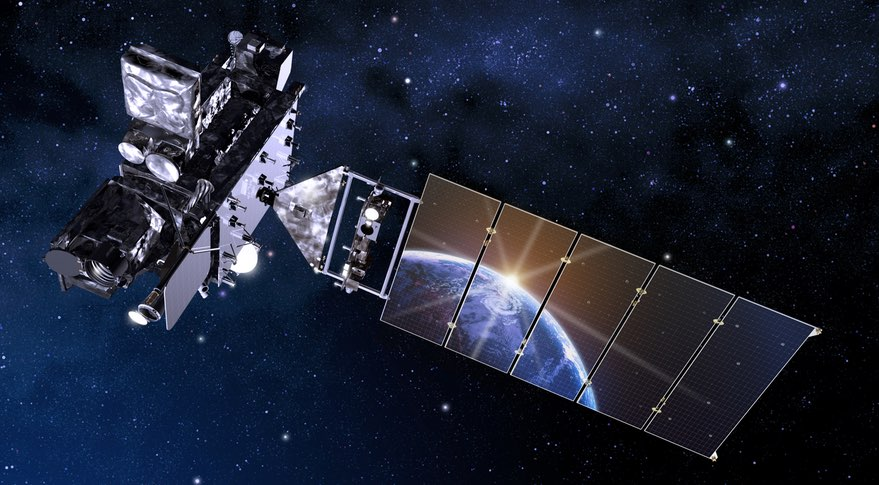
\includegraphics[scale=0.4]{satellite.jpg} 
\end{center}

\end{titlingpage}

\newpage

\tableofcontents

\newpage

\section{NOAA 16 DEB}

\begin{center}
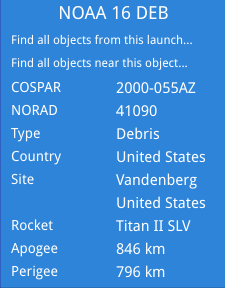
\includegraphics[scale=0.6]{NOAA16DEB.png}
\end{center}

\begin{center}
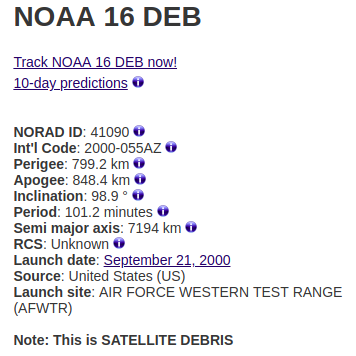
\includegraphics[scale=0.6]{NOAA.png}
\end{center}

\begin{itemize}
\item \textbf{Identificación:} 2000-055AZ
\item \textbf{Tipo de órbita:} LEO (Low Earth Orbit)
\item \textbf{Tipo de satélite y nombre de la constelación:} DEBRIS (limpia basura).
\item \textbf{Cobertura:} No tiene difusión de ninguna señal.
\item \textbf{Altitud:} 7194 km - 6371 km (radio de La Tierra) = 823 km
\item \textbf{Periodo:} 101.2 minutos
\item \textbf{Organización operadora:} United States (US).
\item \textbf{Aplicaciones:} Recolectar basura
\item \textbf{Vida útil:} En el 2019 hace 19 años.
\end{itemize}

\section{COSMOS 2115}

\begin{center}
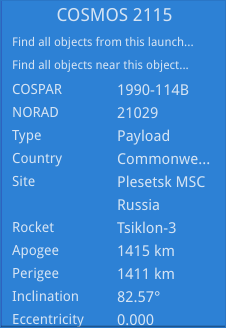
\includegraphics[scale=0.6]{COSMOS2115.png}
\end{center}

\begin{center}
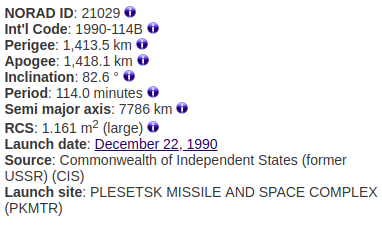
\includegraphics[scale=0.6]{COSMOS.png}
\end{center}

\begin{itemize}
\item \textbf{Identificación:} 1990-114B
\item \textbf{Tipo de órbita:} LEO (Low Earth Orbit)
\item \textbf{Tipo de satélite y nombre de la constelación:} Strela, Strela 3 system
\item \textbf{Cobertura:} Baja
\item \textbf{Altitud:} 7786 km - 6371 km (radio de La Tierra) = 1415 km
\item \textbf{Periodo:} 114 minutos
\item \textbf{Organización operadora:} USSR
\item \textbf{Aplicaciones:} Comunicaciones militares.
\item \textbf{Vida útil:} En el 2019 hace 19 años.
\end{itemize}

\end{document}